\documentclass[12pt,a4paper]{report}
\usepackage[utf8]{vietnam}
\usepackage{amsmath}
\usepackage{amsfonts}
\usepackage{amssymb}
\usepackage{makeidx}
\usepackage{graphicx}
\usepackage{fancybox}
\usepackage{boxedminipage}


\usepackage[framemethod=TikZ]{mdframed}
\newcounter{dinhnghia}[section] \setcounter{dinhnghia}{0}
\renewcommand{\thedinhnghia}{\arabic{section}.\arabic{dinhnghia}}
\newenvironment{dinhnghia}[2][]{%
	\refstepcounter{dinhnghia}%
	\ifstrempty{#1}%
	{\mdfsetup{%
			frametitle={%
				\tikz[baseline=(current bounding box.east),outer sep=0pt]
				\node[anchor=east,rectangle,fill=green!20]
				{\strut Định nghĩa~\thedinhnghia};}}
	}%
	{\mdfsetup{%
			frametitle={%
				\tikz[baseline=(current bounding box.east),outer sep=0pt]
				\node[anchor=east,rectangle,fill=green!20]
				{\strut Định nghĩa~\thedinhnghia~(#1)};}}%
	}%
	\mdfsetup{innertopmargin=10pt,linecolor=green!20,%
		linewidth=2pt,topline=true,%
		frametitleaboveskip=\dimexpr-\ht\strutbox\relax
	}
	\begin{mdframed}[]\relax%
		\label{#2}}{\end{mdframed}}
	
\newcounter{dinhly}[section] \setcounter{dinhly}{0}
\renewcommand{\thedinhly}{\arabic{section}.\arabic{dinhly}}
\newenvironment{dinhly}[2][]{%
	\refstepcounter{dinhly}%
	\ifstrempty{#1}%
	{\mdfsetup{%
			frametitle={%
				\tikz[baseline=(current bounding box.east),outer sep=0pt]
				\node[anchor=east,rectangle,fill=blue!20]
				{\strut Định lý~\thedinhly};}}
	}%
	{\mdfsetup{%
			frametitle={%
				\tikz[baseline=(current bounding box.east),outer sep=0pt]
				\node[anchor=east,rectangle,fill=blue!20]
				{\strut Định lý~\thedinhly~(#1)};}}%
	}%
	\mdfsetup{innertopmargin=10pt,linecolor=blue!20,%
		linewidth=2pt,topline=true,%
		frametitleaboveskip=\dimexpr-\ht\strutbox\relax
	}
	\begin{mdframed}[]\relax%
		\label{#2}}{\end{mdframed}}
	
\usepackage[left=3.50cm, right=2.00cm, top=3.50cm, bottom=3.00cm]{geometry}
\usepackage{scrextend}
\changefontsizes{13pt}
\usepackage{fancyhdr}
\pagestyle{fancy}
\lhead{}
\chead{}
\cfoot{\thepage}
\rfoot{\textit{Toán Tin K61}}
\lfoot{\textit{Các mô hình ngẫu nhiên và ứng dụng}}
\renewcommand{\headrulewidth}{0.4pt}
\renewcommand{\footrulewidth}{0.4pt}
\begin{document}
	\thisfancypage{%đóng khung trang này
		\setlength{\fboxsep}{0pt}% 8pt là độ dày của đường viền
		\fbox}{} % phần nội dung sau là tương tự như đã làm
	\thispagestyle{empty}
	\begin{center}
		\vspace*{0.1cm}
		\fontsize{14}{12}
		\textbf{TRƯỜNG ĐẠI HỌC BÁCH KHOA HÀ NỘI}\\
		\textbf{VIỆN TOÁN ỨNG DỤNG VÀ TIN HỌC}\\
		\textbf{------ o0o ------}
	\end{center}
	\vspace*{0.8cm}
	\begin{center}
		
\includegraphics[scale=.5]{bk.png}
	\end{center}
	\vspace*{0.8cm}
	\begin{center}
		\fontsize{20}{18}
		\textbf{CÁC MÔ HÌNH NGẪU NHIÊN \\VÀ ỨNG DỤNG}\\
		\vspace*{0.8cm}
		\fontsize{18}{16}
		\textbf{HỌC TĂNG CƯỜNG}\\
	\end{center}
	\vspace*{0.7cm}
	\begin{center}
		\fontsize{14}{16}
		\begin{tabular}{ll}		
			\textbf{Giảng viên hướng dẫn:} & \textbf{TS Nguyễn Thị Ngọc Anh} 
		\end{tabular} \\
	\textbf{Nhóm sinh viên thực hiện}\\
	\begin{tabular}{ll}
		\textbf{Hoàng Thanh Lưu} & \textbf{MSSV: 20162602} \\
		\textbf{Lại Thùy Linh} & \textbf{MSSV: 20162401} \\
		\textbf{Nguyễn Hữu Đạt} & \textbf{MSSV: 20160933} \\
	\end{tabular}\\
		\vspace*{2cm}
		\fontsize{14}{16}
		\textbf{Hà Nội - 7/2020}
	\end{center}
\newpage
\chapter*{Lời nói đầu}
Xã hội ngày càng hiện đại, các kỹ thuật công nghệ ngày càng phát triển, đi cùng với nó
là các nghiên cứu phát triển không ngừng về lĩnh vực trí tuệ nhân tạo và học máy, cho ra đời
các hệ thống máy móc thông minh ứng dụng rộng rãi trong hầu hết các lĩnh vực đời sống
như máy truy tìm dữ liệu, chẩn đoán y khoa, phát hiện thẻ tín dụng giả, phân tích thị trường
chứng khoán, phân loại chuỗi DNA, nhận dạng tiếng nói và chữ viết, ... đặc biệt là trong lĩnh vực điều khiển.\\\\
Chúng ta có rất nhiều thuật toán học như học có giám sát, học không có giám sát,
học tăng cường, ... Mỗi loại thuật toán thích ứng với từng loại bài toán cụ thể. Trong báo
cáo này, chúng ta sẽ nghiên cứu và tìm hiểu các vấn đề liên quan đến phương pháp học tăng
cường (Reinforcement Learning). Đây là một thuật toán học có khả năng giải quyết được
những bài toán thực tế khá phức tạp trong đó có sự tương tác giữa hệ thống và môi trường.
Với những tình huống môi trường không chỉ đứng yên, cố định mà thay đổi phức tạp thì các
phương pháp học truyền thống không còn đáp ứng được mà phải sử dụng phương pháp học
tăng cường. Những bài toán với môi trường thay đổi trong thực tế là không nhỏ và ứng dụng
nhiều trong các lĩnh lực quan trọng.\\\\
Xin được gửi lời cảm ơn chân thành nhất tới TS Nguyễn Thị Ngọc Anh - Giảng viên Viện Toán ứng dụng và Tin học vì đã có những nhận xét, góp ý khách quan để nhóm hoàn thành tốt hơn báo cáo này. Dù đã dành nhiều thời gian tìm hiểu, đầu tư nghiêm túc nhưng báo cáo không thể tránh khỏi những sai sót, cả về chủ quan và khách quan. Vì vậy nhóm thực hiện rất mong nhận được sự góp ý quý báu của các bạn sinh viên, các thầy cô giáo để báo cáo trở nên hoàn thiện hơn.\\\\ Nhóm xin chân thành cảm ơn!
\begin{flushright}
	\begin{tabular}{cccc}
		&  Hà Nội tháng  7 năm 2020 && \\ 
		&    Nhóm thực hiện && \\ &    \textit{Hoàng Thanh Lưu} && \\&    \textit{Lại Thùy Linh} && \\&   \textit{Nguyễn Hữu Đạt} && 
	\end{tabular} 
\end{flushright}
\tableofcontents
\chapter{Giới thiệu về học tăng cường}
Trong ngành khoa học máy tính, học tăng cường (Reinforcement Learning) là một lĩnh vực con của học máy, nghiên cứu cách thức một \textit{agent} - tác tử trong một môi trường nên chọn thực hiện các hành động nào để cực đại hóa một khoản thưởng (reward) nào đó về lâu dài. Các thuật toán học tăng cường cố gắng tìm một chiến lược ánh xạ các trạng thái của thế giới tới các hành động mà \textit{agent} nên chọn trong các trạng thái đó.\\\\
Môi trường thường được biểu diễn dưới dạng một quá trình quyết định Markov trạng thái hữu hạn (\textit{Markov Decision Process - MDP}), và các thuật toán học tăng cường cho ngữ cảnh này có liên quan nhiều đến các kỹ thuật quy hoạch động. Các xác suất chuyển trạng thái và các xác suất thu lợi trong MDP thường là ngẫu nhiên nhưng lại tĩnh trong quá trình của bài toán (\textit{stationary over the course of the problem}). \\\\
Khác với học có giám sát, trong học tăng cường không có các cặp dữ liệu vào/kết quả đúng, các hành động gần tối ưu cũng không được đánh giá đúng sai một cách tường minh. Hơn nữa, ở đây hoạt động trực tuyến (\textit{on-line performance}) được quan tâm, trong đó có việc tìm kiếm một sự cân bằng giữa khám phá (lãnh thổ chưa lập bản đồ) và khai thác (tri thức hiện có). Trong học tăng cường, sự được và mất giữa khám phá và khai thác đã được nghiên cứu chủ yếu qua bài toán \textit{multi-armed bandit}.\\\\
Một cách hình thức, mô hình học tăng cường bao gồm:
\begin{itemize}
	\item $S$: tập các trạng thái của môi trường;
	\item $A$: tập các hành động;
	\item $\mathbb{R}$: tập các khoản "thưởng" với giá trị vô hướng.
\end{itemize}
Có hai phương pháp thường được sử dụng để giải các bài toán quyết định đó là tìm kiếm
trong không gian chiến lược và tìm kiếm trong không gian hàm giá trị hay còn gọi là “phép lặp
chiến lược” và “phép lặp giá trị”. Hai phương pháp này chính là các giải thuật học tăng cường
đặc trưng. Bên cạnh đó, trong những nghiên cứu gần đây các nhà khoa học đề xuất một phương
pháp kết hợp giữa hai phương pháp trên đó chính là phương pháp \textit{Actor-Critic learning}.\\\\
Các thuật toán học tăng cường được chia thành hai loại chính đó là: học dựa trên mô hình
(\textit{model-based}) và học không có mô hình hay nói cách khác họ tự do (\textit{model-free}). Đại điện cho
kiểu học dựa trên mô hình phải kể đến phương pháp quy hoạch động (\textit{Dynamic Programming}), còn đại diện cho kiểu học không có mô hình là phương pháp \textit{Monte Carlo} và phương pháp TD (\textit{Temporal Difference}).\\\\
Các chủ đề nghiên cứu hiện tại bao gồm: Cách biểu diễn khác (chẳng hạn cách tiếp cận \textit{Predictive State Representation} - biểu diễn trạng thái tiên đoán), tìm kiếm leo đồi trong không gian chiến lược, các kết quả hội tụ đối với mẫu nhỏ, các thuật toán và kết quả hội tụ cho các MDP quan sát được một phần (\textit{partially observable MDP}), học tăng cường môdun và phân cấp (\textit{modular and hierarchical}). Gần đây, học tăng cường đã được áp dụng trong lĩnh vực Tâm lý học để giải thích quá trình học và hoạt động của con người.

\chapter{Phương pháp}
\section{Nhắc lại về quá trình Markov}
\subsection{Xích Markov}
\begin{dinhnghia}[Xích Markov]{ding:dinhnghia1}
	Dãy biến ngẫu nhiên  ${(X_n)}_{n \geq 0}$ được gọi là một xích Markov với phân phối ban đầu $\lambda$ và ma trận chuyển $P$ nếu
	\begin{itemize}
	\item[i)] $X_0$ có phân phối $\lambda$, tức là $$\mathbb{P} (X_0 = i) = \lambda_i, \qquad \forall i \in I;$$
	\item[ii)] Với mọi $n \geq 0$, phân phối của $X_{n+1}$ với điều kiện $X_n = i_n$ là $(p_{i_nj})_{j \in I}$ và độc lập với $X_0,. . .,X_{n-1}$, tức là \begin{equation}
	\mathbb{P}(X_{n+1} = i_{n+1} | X_n = i_n, . . ., X_0 = i_0) = \mathbb{P}(X_{n+1} = i_{n+1} | X_n=i_n) = p_{i_ni_{n+1}} \nonumber
	\end{equation} với mọi $n \geq 0$ và $i_0,..., i_{n+1} \in I.$
	\end{itemize}
$X_n$ được gọi là trạng thái của xích Markov tại thời điểm thứ $n$.
	
\end{dinhnghia}
\subsection{Quá trình Markov}
Xét họ các biến ngẫu nhiên $X(t)_{t \geq 0}: $
\begin{itemize}
	\item $T$ là tập hợp chỉ thời gian rời rạc nếu quá trình Markov xét với thời gian rời rạc. Khi quá trình Markov xét với thời gian liên tục thì $T$ là tập hợp chỉ thời gian liên tục.
	\item $I$ là không gian trạng thái rời rạc nếu xích Markov có thời gian rời rạc hoặc liên tục. $I$ là không gian trạng thái liên tục khi xét quá trình Markov.
\end{itemize}
\begin{dinhnghia}[Quá trình Markov]{ding:dinhnghia1}
$(X_t)_{t\geq 0}$ với không gian trạng thái hữu hạn $I$ được gọi là quá trình Markov nếu với mọi $t_1 < t_2 < ... < t_n$ và mọi $i_1, i_2, ..., i_n \in I$ thì   $$\mathbb{P}(X_t = i|X_{t_1} = i_1, ..., X_{t_n} = i_n) = \mathbb{P}(X_{t} = i|X_{t_n} = i_n)$$
\end{dinhnghia}

\begin{dinhnghia}[Quá trình Markov thuần nhất]{ding:dinhnghia1}
	Cho $(X_t)_{t\geq 0}$ là quá trình Markov, và $$\forall h > 0, p(s + h, i, s+t+h, j = p (s,i, s+t,j) = p_{ij}(t))$$ khi đó quá trình Markov được gọi là quá trình Markov thuần nhất.
\end{dinhnghia}

\section{Quá trình quyết định Markov (MDP)}
Quá trình quyết định Markov (MDP) cung cấp một nền tảng toán học cho việc mô hình
hóa ra quyết định trong các tình huống mà kết quả có yếu tố ngẫu nhiên và/hoặc phụ thuộc
vào sự điều khiển của một người ra quyết định. MDP được sử dụng rất nhiều các lĩnh vực
khác nhau, bao gồm robot, điều khiển tự động, kinh tế, chế tạo, . . . Trong phần này, chúng ta
sẽ trình bày về quá trình quyết định Markov trong đó tập trung vào các khái niệm của quá
trình Markov có số bước vô hạn và hữu hạn.
\subsection{Quá trình quyết định Markov là gì?}
Một quá trình quyết định Markov là một quá trình điều khiển ngẫu nhiên thời gian rời rạc. Tại mỗi bước thời gian, quá trình này trong một vài trạng thái $s$, và người ra quyết định có thể chọn bất kỳ hành động $a$ nào có hiệu lực trong trạng thái $s$. Quá trình này đáp ứng tại bước thời gian tiếp theo bằng cách di chuyển ngẫu nhiên vào một trạng thái mới $s'$, và đưa ra cho người ra quyết định một phần thưởng tương ứng $R_a(s, s')$. \\\\ Xác suất mà quá trình di chuyển vào trạng thái mới của nó $s'$ bị ảnh hưởng bởi hành động được chọn. Đặc biệt, nó được đưa ra bởi hàm chuyển tiếp trạng thái $P_a(s, s')$. Do đó, trạng thái kế tiếp $s'$ phụ thuộc vào trạng thái hiện tại $s$ và hành động của người ra quyết định $a$. Nhưng  $s$ và $a$ đã cho, lại độc lập có điều kiện với toàn bộ trạng thái và hành động trước đó; nói cách khác, các trạng thái chuyển tiếp của một quá trình MDP thỏa mãn thuộc tính Markov.
\begin{dinhnghia}[Quá trình quyết định Markov]{ding:dinhnghia1}
Một quá trình quyết định Markov là một tập 5-dữ liệu $(S, A, P_.(.,.), R_.(.,.), \gamma)$ trong đó
\begin{itemize}
	\item $S$ là một tập hữu hạn các trạng thái, kí hiệu $S_t$ là trạng thái tại thời điểm $t$.
	\item $A$ là một tập hữu hạn các hành động (ngoài ra, $A_s$ là tập hữu hạn các hành động có sẵn từ trạng thái $s$ với $s \in S$), kí hiệu $A_t$ là hành động tại thời điểm $t$.
	\item $P_a(s, s') = Pr(s_{t+1} = s'|s_t = s, a_t = a)$ là xác suất mà hành động $a$ trong trạng thái $s$ tại thời gian $t$ sẽ dấn đến trạng thái $s'$ tại thời gian $t+1$. 
	\item $R_a(s, s')$ là phần thưởng trực tiếp (hoặc phần thưởng trực tiếp mong đợi) nhận được sau khi chuyển tiếp sang trạng thái $s'$ từ trạng thái $s$.
	\item $\gamma \in [0, 1]$ là hệ số chiết khấu, sẽ đại diện cho sự khác biệt quan trọng giữa các phần thưởng tương lai và các phần thưởng hiện tại.  
\end{itemize}
\end{dinhnghia}
\begin{figure}[h]
	\centering
	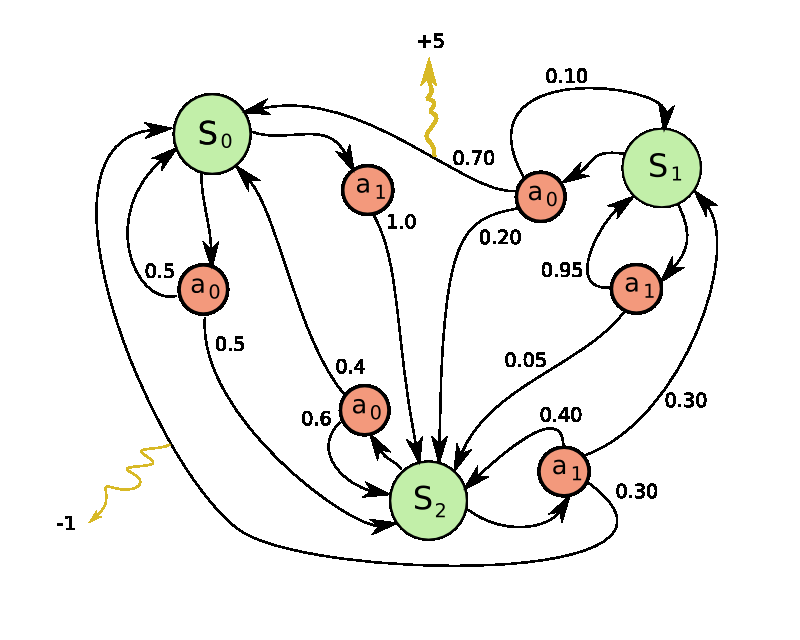
\includegraphics[scale=.5]{1}
	\caption{Ví dụ về một MDP đơn giản với ba trạng thái và hai hành động.}
\end{figure}

\begin{dinhnghia}[Chiến lược quyết định]{ding:dinhnghia1}
Một chiến lược $\pi$ là một phân phối các hành
động tại mỗi trạng thái $$\pi(a|s) = Pr[A_t=a|S_t = s]$$ Một số kiểu chiến lược như sau
\begin{itemize}
	\item $\pi = (\pi^0, ..., \pi^{T-1})$ được gọi là một chiến lược Markov nếu tại mỗi thời điểm $n$, quyết
	định $\pi^n$ không phụ thuộc vào quá khứ $h_{n-1}$. Ví dụ $$\pi^n_{h_{n-1}, i_n} (a) = \pi^n_{h^{'
		}_{n-1}, i_n}(a), a \in A(i_n), i_n \in S \text{ } \forall h_{n-1}, h^{'
	}_{n-1}$$
\item $\pi$ được gọi là một chiến lược dừng nếu mọi quy tắc quyết định đều bằng nhau $$\pi^n = \pi^0 ; \quad n = 0,1,...,T-1$$
\end{itemize}
\end{dinhnghia}
Trong quá trình quyết định Markov, mỗi chiến lược xác định đầy đủ hành động của một tác
nhân. Ngoài ra, các chiến lược này chỉ phụ thuộc vào trạng thái của xích Markov tại thời
điểm hiện tại (không phụ thuộc vào quá khứ).
\subsection{Bài toán quyết định Markov}
\subsubsection{a. Bài toán}
Bài toán quyết định Markov là bài toán học từ các tác động để đạt được mục đích. Người
học và người ra quyết định được gọi là tác tử. Tất cả những gì mà chúng tương tác với, bao
gồm mọi thứ bên ngoài tác tử được gọi là môi trường. Các tác động thực hiện một cách liên
tục, tác tử lựa chọn hành động, môi trường đáp ứng lại các hành động đó và chuyển từ trạng
thái hiện thời sang trạng thái mới. Môi trường cũng đem lại các mục tiêu, các giá trị hằng số
mà tác tử cố gắng cực đại hóa qua thời gian. Một đặc tả hoàn thiện về môi trường được coi là
một "nhiệm vụ", một thực thể của bài toán quyết định Markov.\\\\
Tóm lại, bài toán quyết định Markov liên quan đến lớp bài toán trong đó một tác tử rút ra kết
luận trong khi phân tích một chuỗi các hành động của nó cùng với tín hiệu vô hướng được
đưa ra bởi môi trường.\\\\
Trong khái niệm chung này, có thể thấy hai đặc tính quan trọng:
\begin{itemize}
	\item Tác tử tương tác với môi trường và cặp "tác tử + môi trường" tạo thành một hệ thống
	động.
	\item Tín hiệu tăng cường, được nhận biết dựa vào mục tiêu, cho phép tác tử thay đổi hành
	vi của nó.
\end{itemize}
Lược đồ tương tác tác tử-môi trường như sau:
\begin{figure}[h]
	\centering
	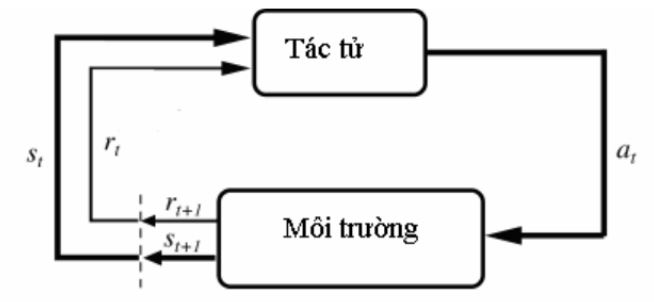
\includegraphics[scale=.5]{2} 
	\caption{Mô hình tương tác giữa tác tử và môi trường}
\end{figure}\\
Trong lược đồ trên, tác tử và môi trường tác động lẫn nhau tại mỗi bước trong chuỗi các
bước thời gian rời rạc, $t = 0,1,2,3,...$. Tại mỗi bước thời gian $t$, tác tử nhận một số biểu diễn về trạng thái của môi trường, $s_t \in S$ với $S$ là tập các trạng thái có thể, và trên đó lựa chọn một
hành động $a_t\in A(s_t)$, với $A(s_t)$ là tập các hành động trong trạng thái $s_t$. Mỗi bước thời gian
tiếp theo, tác tử nhận một giá trị tăng cường $r_{t+1} \in R$ và tự nó tìm ra một trạng thái mới $s_{t+1}$.
Tại mỗi bước tác tử thực hiện ánh xạ từ các trạng thái đến các hành động có thể lựa chọn. \\
Phép ánh xạ này được gọi là chiến lược của tác tử, kí hiệu là $\pi_t$ với $\pi_t(s, a)$ là xác suất thực
hiện hành động $a_t = a$ khi $s_t = s$.\\\\Như vậy bài toán quyết định Markov thực chất có thể được phát biểu như sau
\begin{center}
	\begin{tabular}{l|l}
		\textbf{Input} & Tập các trạng thái $S$ \\ &Tập các hành động có thể $A$ \\ & Tập các tín hiệu tăng cường (mục tiêu) \\
		\hline
		\textbf{Output} & $\pi : S \to A$ sao cho $R$ lớn nhất
	\end{tabular}
\end{center}
\subsubsection{b. Các phần tử của bài toán quyết định Markov}
Dựa vào tác tử và môi trường, chúng ta có thể định nghĩa các phần tử con của một bài
toán quyết định Markov: chiến lược (\textit{policy}), hàm phản hồi (\textit{reward function}), hàm giá trị
(\textit{value function}), và không bắt buộc, một mô hình về môi trường.
\begin{itemize}
	\item \textbf{Chiến lược:} Chiến lược định nghĩa cách thức tác tử học từ hành động tại thời điểm đưa ra. Chiến lược
	là một ánh xạ từ tập các trạng thái của môi trường đến tập các hành động được thực hiện khi
	môi trường ở trong các trạng thái đó. Nó tương ứng với tập các luật nhân quả trong lĩnh vực
	tâm lý học. Trong một số trường hợp, chiến lược có thể là một hàm đơn giản hoặc một bảng
	tra cứu, trong những trường hợp khác, nó có thể liên quan đến các tính toán mở rộng, ví dụ
	như một tiến trình tìm kiếm. Chiến lược là nhân của một tác tử với nhận thức rằng một mình
	nó đủ quyết định hành động.
	\item \textbf{Hàm phản hồi:} 
	Mục đích của tác tử là cực đại hóa các mục tiêu được tích lũy trong tương lai. Hàm phản
	hồi $R(t)$ được biểu diễn dưới dạng hàm số đối với các mục tiêu. Trong các bài toán quyết
	định Markov, hàm phản hồi sử dụng biểu thức dạng tổng. Các nhà nghiên cứu đã tìm ra hai
	biểu diễn thường được sử dụng của hàm phản hồi:
	\begin{itemize}
		\item \textit{Trong các bài toán số bước hữu hạn: } Với những bài toán này ta có một số hữu hạn các bước trong tương lai. Sẽ tồn tại một
		trạng thái kết thúc và một chuỗi các hành động giữa trạng thái đầu tiên và trạng thái
		kết thúc được gọi là một giai đoạn. Ta có: $$R(t) = r_t + r_{t+1} + ... + r_{t+K-1}$$ Trong đó $K$ là số các bước trước trạng thái kết thúc.
		\item \textit{ Trong các bài toán số bước vô hạn: } Với những bài toán này ta có chuỗi các hành động là vô hạn. Một hệ số suy giảm
		$\gamma, 0\leq\gamma 
		\leq 1 $ được đưa ra và hàm phản hồi được biểu diễn dưới dạng tổng của các giá
		trị mục tiêu giảm dần: $$R(t) = \sum_{k=0}^{\infty}\gamma^kr_{t+k}$$
		Hệ số $\gamma$ cho phép xác định mức độ ảnh hưởng của những bước chuyển trạng thái tiếp
		theo đến giá trị phản hồi tại thời điểm đang xét. Giá trị của $\gamma$ cho phép điều chỉnh giai
		đoạn tác tử lấy các hàm tăng cường. Nếu $\gamma$ = 0, thì tác tử chỉ xem xét mục tiêu gần
		nhất, giá trị $\gamma$ càng gần với 1 thì tác tử sẽ quan tâm đến các mục tiêu xa hơn trong tương
		lai. Như vậy, thực chất bài toán quyết định Markov trong trường hợp này chính là việc
		lựa chọn các hành động để làm cực đại biểu thức $R$: $$R = r_0 + \gamma r_1 + \gamma^2r_2 + \cdots; \quad 0 < \gamma < 1$$
	\end{itemize}
\item \textbf{Hàm giá trị:} Trong mọi trạng thái $s_t$, một tác tử lựa chọn một hành động dựa theo một chiến lược điều
khiển, $\pi: a_t = \pi(s_t)$. Hàm giá trị tại một trạng thái của hệ thống được tính bằng kỳ vọng toán
học của hàm phản hồi theo thời gian. Hàm giá trị là hàm của trạng thái và xác định mức độ
thích hợp của chiến lược điều khiển $\pi$ đối với tác tử khi hệ thống đang ở trạng thái $s$. Hàm
giá trị của trạng thái $s$ trong chiến lược $\pi$ được tính như sau $$V^{\pi}(s) = E_{\pi}\{R_t|s_t=s\}$$ Bài toán tối ưu bao gồm việc xác định chiến lược điều khiển $\pi^*$ sao cho hàm giá trị của trạng
thái hệ thống đạt cực đại sau một số vô hạn hoặc hữu hạn các bước $$\pi^* = \{\pi_0(s_0), \pi_1(s_1), \cdots,\pi_{N-1}(s_{N-1})\}$$
Đối với bài toán có số bước vô hạn ta có hàm giá trị trạng thái $$V^{\pi}(s) = E_{\pi}\{R_t = \sum_{k=0}^{\infty}\gamma^kr_{t+k+1|s_t = s}\}$$ Sử dụng các phép biến đổi
\begin{eqnarray}
	V^\pi(s) & = & E_{\pi}\{R_t|s_t=s\}\nonumber \\ &=& E_{\pi} \bigg\{\sum_{k=0}^{\infty}\gamma^kr_{t+k+1}|s_t = s\bigg\}\nonumber \\ &=& E_{\pi}\bigg\{r_{t+1}+\gamma\sum_{k=0}^{\infty}\gamma^kr_{t+k+2}|s_t=s\bigg\} \nonumber\\&=& \sum_{a}\pi(s, a)\sum_{s'}P^a_{ss'}\bigg[R^a_{ss'} + \gamma E_{\pi}\bigg\{\sum_{k=0}^{\infty}\gamma^kr_{t+k+2}|s_{t+1} = s'\bigg\}\bigg] \nonumber \\ &=& \sum_{a}\pi(s, a) \sum_{s'}P^a_{ss'}[R^a_{ss'} + \gamma V^{\pi}(s')] \nonumber
\end{eqnarray} Như vậy, hàm $V^{\pi}(s)$ có thể được viết lại một cách đệ qui như sau $$V^{\pi}(s) = E_{\pi}r_{t+1} + \gamma V^{\pi}(S_{t+1})|S_t = s$$ hay \begin{equation}
	V^{\pi}(s) = R(s, a) + \gamma\sum_{s'\in S}P^a_{ss'}V^{\pi}(s')
\end{equation}
Với $P^a_{ss'}$ là xác suất để chuyển từ trạng thái $s$ sang $s'$ khi áp dụng hành động $a$. Chúng ta có
thể tính toán hàm $V^{\pi}(s)$ ngoại tuyến nếu biết trạng thái bắt đầu và xác suất mọi phép chuyển
đổi theo mô hình. Vấn đề đặt ra là sau đó giải quyết hệ thống các phương trình tuyến tính
trong công thức (2.1). Chúng ta biết rằng tồn tại một chiến lược tối ưu, kí hiệu $\pi^*$, được định
nghĩa như sau 
\begin{equation}
	\begin{split}
	V^{\pi^*}(s) \geq V^{\pi}(s) \nonumber\\ \pi^* = argmax_{\pi}V^{\pi}(s)\nonumber
	\end{split}
\end{equation} để đơn giản chúng ta viết $V^* = V^{\pi^*}$. Hàm giá trị tối ưu của một trạng thái tương ứng với
chiến lược tối ưu là $$V^{\pi}(s) = \max_{\pi}V^{\pi}(s)$$ đây là phương trình tối ưu \textit{Bellman} (hoặc phương trình của quy hoạch động) ta sẽ nói chi tiết
hơn ở phần tiếp theo.\\\\Tóm lại $V^{\pi}$ là hàm giá trị trạng thái cho chiến lược $\pi$. Giá trị của trạng thái kết thúc
thường bằng 0. Tương tự, định nghĩa $Q^{\pi}(s, a)$ là giá trị của việc thực hiện hành động $a$ trong
trạng thái $s$ dưới chiến lược điều khiển $\pi$, được tính bằng kỳ vọng toán học của hàm phản hồi
bắt đầu từ trạng thái $s$, thực hiện hành động $a$ trong chiến lược $\pi$ $$Q^{\pi}(s, a) = E_{\pi}\{R_t|s_t = s, a_t = a\} = E_{\pi}\bigg\{\sum_{k=0}^{\infty}\gamma^kr_{t+k+1}|s_t=s, a_t=a\bigg\}$$ $Q^{\pi}$ được gọi là hàm giá trị hành động cho chiến lược $\pi$. Và các hàm giá trị $V^{\pi
}$, $Q^{\pi}$ có thể
được ước lượng từ kinh nghiệm.
\end{itemize}
\subsection{Phương trình tối ưu Bellman cho bài toán MDP}
Từ trạng thái $s$, có thể đưa ra nhiều hành động khác nhau và mỗi chiến lược xác định một
phân phối xác suất của hành động đó, do đó, sử dụng phương trình tối ưu Bellman để đưa ra
quyết định cho bài toán này.\\
Phương trình Bellman cho hàm giá trị trạng thái
\begin{eqnarray}
	V^{\pi}(s) &=& R_{\pi}(s) + \gamma \sum_{s'\in S} P_{\pi}(s, s')V^{\pi}(s') \nonumber \\ &=& \sum_{a \in A}\pi(a|s)\bigg(R_a(s) + \gamma\sum_{s'\in S}P_{\pi}(s, s')V^{\pi}(s')\bigg) \nonumber
\end{eqnarray}
Phương trình Bellman cho hàm giá trị hành động $$Q^{\pi}(s, a) = R_a(s) + \gamma \sum_{s'\in S}P_a(s, s')\sum_{a' \in A}\pi(a'|s')Q^{\pi}(s', a')$$
\newpage
\begin{dinhnghia}{ding:dinhnghia1}
	Hàm giá trị trạng thái tối ưu $V^*(s)$ là hàm trả về trạng thái tối ưu trên tất
	cả các chiến lược $$V^*(s) = \max_{\pi}V^{\pi}(s)$$
\end{dinhnghia}

\begin{dinhnghia}{ding:dinhnghia1}
	Hàm giá trị hành động tối ưu $Q^*(s, a)$ là hàm trả về các hành động tối ưu
	trên tất cả các chiến lược $$Q^*(s, a) = \max
	_{\pi}Q^{\pi}(s, a)$$
\end{dinhnghia}

\begin{dinhnghia}{ding:dinhnghia1}
	$\pi$ được gọi là chiến lược tối ưu nếu $V^{\pi}(s) \geq V^{\pi'}(s), \forall s.$
	Xác định một chiến lược tối ưu: Một chiến lược tối ưu có thể được xác định bằng cách tìm
	hàm cực đại $Q^*(s, a)$ $$ \pi^*(a|s) = \begin{cases}
	1 & \text{ nếu } a = argmax_{a\in A} Q^*(s, a) \\ 0 &  \text{ ngược lại }
	\end{cases}$$
\end{dinhnghia}
Phương trình tối ưu Bellman cho $V^{*}(s)$ $$V^*(s) = \max
_aR_a(s) + \gamma \sum_{s'\in S} P_a(s, s')V^{*}(s')$$
Phương trình tối ưu Bellman cho $Q^*(s, a)$ $$Q^*(s, a) = R_a(s) + \gamma\sum_{s'\in S}P_a(s, s')\max_{a'}Q^*(s', a')$$ Phương trình tối ưu Bellman là một phương trình phi tuyến có thể giải bằng một số phương
pháp: lặp giá trị và lặp chính sách.
\section{Thuật toán Q-Learning}
\subsection{Giới thiệu}
Q-Learning là một thuật toán học tăng cường không mô hình. Mục tiêu của Q-Learning là học một chính sách, chính sách cho biết máy sẽ thực hiện hành động nào trong hoàn cảnh nào. Nó không yêu cầu một mô hình (do đó hàm ý "không mô hình") của môi trường và nó có thể xử lý các vấn đề với chuyển đổi và phần thưởng ngẫu nhiên, mà không cần điều chỉnh. \\\\ Đối với bất kỳ quá trình quyết định Markov hữu hạn nào, Q-Learning tìm một chính sách tối ưu theo nghĩa là nó tối đa hóa giá trị mong đợi của tổng số phần thưởng trên bất kỳ và tất cả các bước tiếp theo, bắt đầu từ trạng thái hiện tại. Q-Learning có thể xác định một chính sách lựa chọn hành động tối ưu cho bất kỳ quá trình quyết định Markov hữu hạn cụ thể nào, với thời gian thăm dò vô hạn và chính sách một phần ngẫu nhiên. "Q" đặt tên theo tên hàm phần thưởng trả về, được sử dụng để cải thiện hoạt động và có thể nói là đại diện cho "chất lượng" của một hành động được thực hiện trong một trạng thái nhất định.
\subsection{Thuật toán Q-Learning}
Cho một chiến lược (\textit{policy}) $\pi$, ta viết lại công thức về Q-value
(hay là giá trị hành động) như sau \begin{equation}
	Q^{\pi}(s, a) = R(s, a) + \gamma\sum_{s'\in S} P^a_{ss'}V^{\pi}(s')
\end{equation}
Trong công thức (2.2), $Q^{\pi}(s, a)$ là Q-value khi thực hiện hành động $a$ tại trạng thái $s$ theo chiến
lược $\pi$; $R(s,a)$ là phần thưởng nhận được; $s'$ là trạng thái kế tiếp. $\gamma$ là hệ số giảm (\textit{discount
rate}), đảm bảo "gần" đích Q-value càng lớn. \\\\ Nói các khác, Q-value là hàm giá trị hành động mong đợi cho việc thực hiện hành động $a$ ở
trạng thái $s$ và tuân theo chính sách $\pi$ sau đó. Mục đích của Q-learning là ước lượng Q-values
cho một chiến lược tối ưu. Để tiện lợi, ta định nghĩa như sau $Q^*(s, a) \equiv Q^{\pi^*}(s, a), \forall s, a.$ Thật
đơn giản để chỉ ra rằng $V^*(s) = \max_aQ^*(s, a)$ và nếu $a^*$ là một hành động mà tại đó mức tối
đa đạt được, sau đó một chiến lược tối ưu có thể được hình thành như $\pi^*(s) \equiv a^*$. Ở đây, lợi
ích của những giá trị Q-value là nếu một tác tử (agent) có thể học chúng, nó có thể dễ dàng
quyết định đâu là tối ưu để hành động. Mặc dù có thể có nhiều hơn một chiến lược tối ưu hay
$a^*$, những giá trị $Q^*$ là duy nhất. \\\\ Trong Q-learning, kinh nghiệm của tác tử (agent) bao gồm một chuỗi tuần tự các quá
trình riêng biệt (gọi là Episodes). Trong episode thứ $n$, tác tử sẽ:
\begin{itemize}
	\item Quan sát trạng thái hiện tại của nó $s_n$, 
	\item  Lựa chọn và thực hiện một hành động $a_n$,
	\item Quan sát trạng thái tiếp theo $s_{n+1}$,
	\item Nhận được ngay phần thưởng $r_n$, và
	\item Điều chỉnh các giá trị $Q_{n-1}$ của nó bằng cách sử dụng hệ số học $\alpha_n$, theo: 
	\begin{equation}
		Q_n(s, a) = \begin{cases}
		(1-\alpha_n)Q_{n-1}(s, a) + \alpha_n[r_n + \gamma V_{n-1}(s_{n+1})] & \text{ nếu } s=s_n, a = a_n, \\ Q_{n-1}(s, a) & \text{ trường hợp khác }
		\end{cases}
	\end{equation}
\end{itemize} Trong đó \begin{equation}
V_{n-1}(s) \equiv \max_bQ_{n-1}(s, b)
\end{equation}
là tốt nhất mà tác tử có thể làm được từ trạng thái $s$. Dĩ nhiên, ở những giai đoạn đầu việc học
thì Q-value có thể không phản ánh đúng chiến lược mà chúng đã được biết (việc tối đa hóa
các hành động ở phương trình (2.3)). Hiển nhiên là các giá trị Q-value ban đầu, $Q_0(s, a)$, cho
tất cả các trạng thái và hành động đã được giả thiết. Ngoài ra ta có thêm giả thiết một bảng
tra cứu (\textit{look-up table}) biểu diễn cho $Q_n(s, a)$. Phân tích thuật toán Q-Leaning, ta có các bước như sau: \begin{enumerate}
	\item Khởi tạo bảng $Q$ với các số 0 và giá trị $Q$ thành các hằng số tùy ý.
	\item Khám phá các hành động: đối với mỗi thay đổi về trạng thái, chọn bất kỳ một hành
	động $a$ nào trong số tất cả các hành động có thể có cho trạng thái hiện tại $S$.
	\item Đi đến trạng thái tiếp theo $S'$ là kết quả của hành động $a$.
	\item Đối với tất cả các hành động có thể từ trạng thái $S'$, hãy chọn một hành động có
	giá trị $Q$ cao nhất.
	\item Cập nhật giá trị bảng $Q$ bằng phương trình.
	\item  Đặt trạng thái tiếp theo làm trạng thái hiện tại.
	\item Nếu trạng thái cuối đạt được, sau đó kết thúc và lặp lại quá trình.
\end{enumerate} 
\begin{figure}[h]
	\centering
	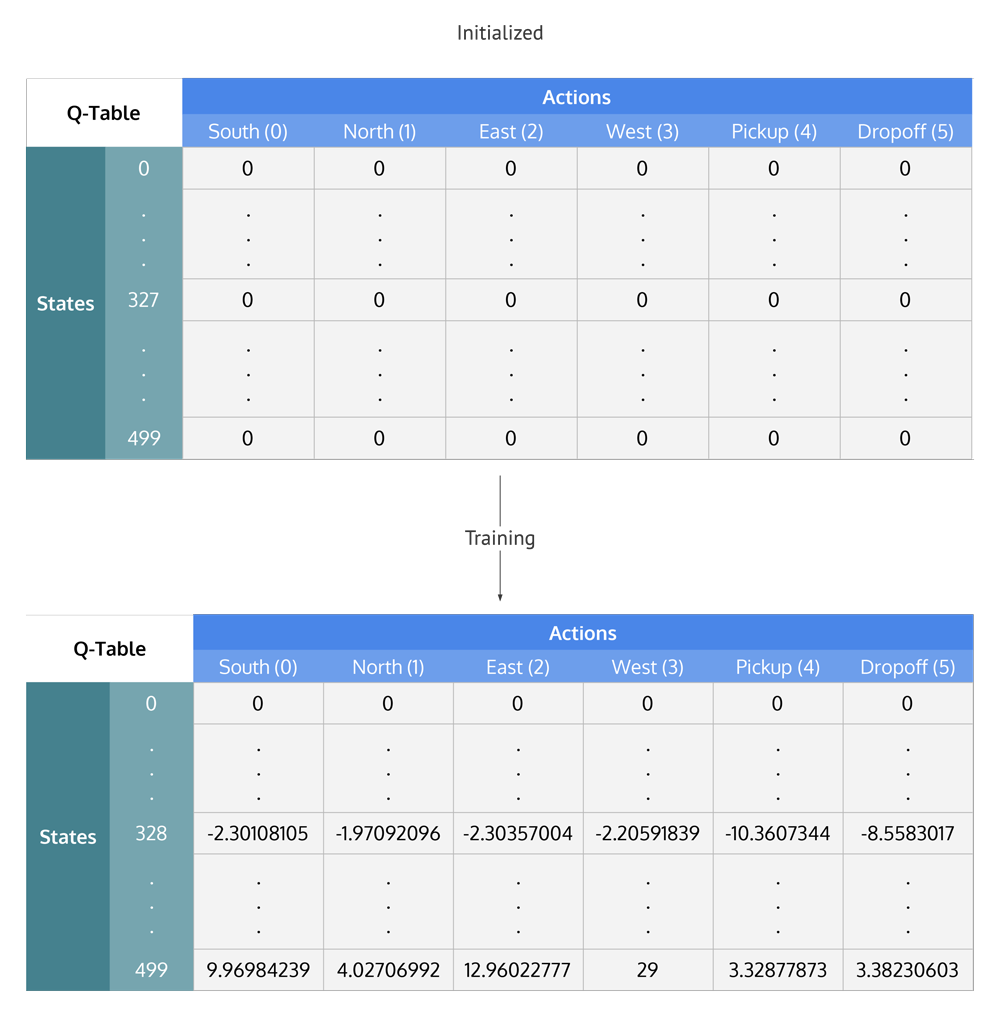
\includegraphics[scale=.3]{3}
	\caption{Bảng Q-Learning về các trạng thái được khởi tạo thành 0, sau đó mỗi ô được cập nhật thông qua đào tạo.}
\end{figure}
\subsection{Sự hội tụ của thuật toán Q-Learning}
Điều kiện quan trọng nhất trong định lý hội tụ được đưa ra dưới đây là chuỗi các quá trình
(Episodes) hình thành nền tảng học tập phải bao gồm vô hạn quá trình cho mỗi trạng thái và
hành động bắt đầu. Đây có thể được coi là một điều kiện mạnh về cách lựa chọn các trạng
thái và hành động, tuy nhiên, trong các điều kiện ngẫu nhiên của định lý, không có phương
pháp nào có thể được đảm bảo để tìm ra một chiến lược tối ưu trong các điều kiện yếu hơn.
Tuy nhiên, xin lưu ý rằng các quá trình không cần phải tạo thành một chuỗi liên tục, đó là $y$
của một quá trình không cần phải là $x$ của quá trình tiếp theo.  Định lý dưới đây định nghĩa một tập các điều kiện theo đó $Q_n(s, a) \to Q^*(s, a)$ khi $n \to \infty$.
Định nghĩa $n^i(s, a)$ là chỉ số của lần thứ $i$ mà hành động $a$ được thử ở trạng thái $s$. 

\begin{dinhly}[Định lý hội
	tụ thuật toán Q-Learning]{dily:dinhly1}
	Cho một miền phần thưởng bị chặn $r_n \leq R$, tỉ lệ học $0 \leq \alpha_n < 1$ và $$\sum_{i=1}^{\infty}\alpha_{n^i(s, a)} = \infty, \sum_{i=1}^{\infty}[\alpha_{n^i (s, a)}]^2 < \infty, \forall s, a$$ thì $Q_n(s, a) \to Q^*(s, a)$ khi n $\to$ $\infty, \forall x, a$ với xác suất bằng 1.
\end{dinhly}

\section{Thuật toán Deep Q-Learning}
Mục đích của bài toán là chọn ra hành động (\textit{action}) thích hợp cho một trạng thái nào đó
(\textit{state}) nào đó. Hay nói cách khác, với \textit{state} là đầu vào và cần đầu ra là một hành động. Công
việc đó sẽ được thực hiện qua một mạng nơ-ron (\textit{Neural Network-NN}). Những gì ta cần làm
chỉ là bỏ đi bảng tra cứu \textit{lookup table} $Q(s,a)$ và thay thế bằng một mạng nơ-ron đơn giản.
Điều đó được mô tả trong Hình 2.4.
\begin{figure}[h]
	\centering
	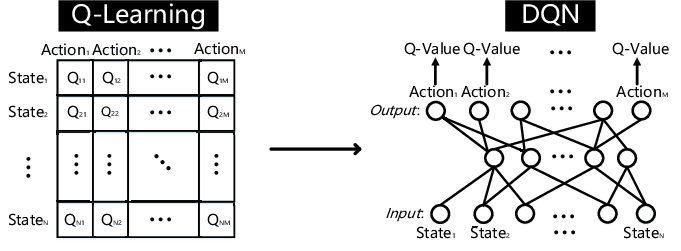
\includegraphics[scale=.6]{4}
	\caption{So sánh về cấu trúc giữa Q-learning và Deep Q-learning}
\end{figure}
\subsection{Hàm mất mát}
Mục đích của ta là bắt mạng học được cách ước lượng Q-Value cho các hành động một
cách chính xác nên đương nhiên hàm mất mát phải tính được sai số giữa Q-value thực tế và
dự đoán. Hàm mất mát định nghĩa dưới dạng đầy đủ như sau: $$Loss = (r+\gamma\max_{a'}Q(s', a'; \theta') - Q(s, a; \theta))^2$$
\subsection{Kinh nghiệm chơi lại (Experience replay)}
Ở phần trên ta đã định nghĩa một mạng nơ-ron lấy \textit{input} là \textit{state} hiện tại và \textit{output} các
Q-value. Thế nhưng nếu mạng nơ-ron cứ liên tục bị đẩy vào từng \textit{state} một sẽ rất dễ bị
\textit{overfitting}vì các \textit{states} liên tục thường giống nhau hoặc có tính tuyến tính (ví dụ: liên tục đi
thẳng/sang trái/phải). Kỹ thuật \textit{Experience Replay} được sử dụng để loại bỏ vấn đề này. Thay
vì mỗi \textit{state} mạng \textit{update} một lần, ta lưu lại các \textit{states} vào bộ nhớ (\textit{memory}). Sau đó thực
hiện \textit{sampling} thành các \textit{batch} nhỏ đưa vào mạng nơ-ron học. Việc này giúp đa dạng hóa
\textit{input} và tránh mạng nơ-ron bị \textit{overfitting}.
\subsection{Mô hình}
Mô hình đầy đủ của Deep Q-Learning được mô tả trong Hình 2.5
\begin{figure}[h]
	\centering
	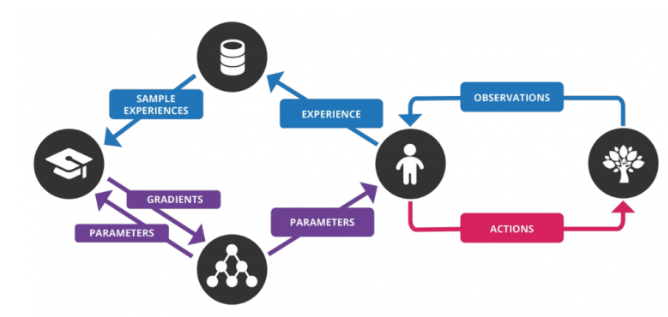
\includegraphics[scale=1]{6}
	\caption{Mô hình đầy đủ Deep Q-Learning}
\end{figure}\\
Tóm lại, Deep Q-Learning thực hiện các bước sau
\begin{enumerate}
	\item \textit{Enviroment} đưa vào mạng một \textit{state} $s$; đầu ra là các Q-value của các \textit{actions} tương
	ứng.
	\item \textit{Agent} chọn \textit{action} bằng một \textit{Policy} và thực hiện \textit{action} $a$ đó.
	\item \textit{Environment} trả lại \textit{state} $s'$ cùng với \textit{reward} $r$ tương ứng và lưu lại \textit{experience} $s, a, r,
	s'$.
	\item Thực hiện \textit{sample} các \textit{experience} thành một vài \textit{batches} và tiến hành luyện mạng.
	\item Lặp lại đến khi kết thúc $M$ \textit{episodes}.
\end{enumerate}
\chapter{Ứng dụng trong thực tế}
\section{Một số ứng dụng thực tế}
Ứng dụng của Học tăng cường trong thực tế cực kỳ đa dạng, trong bất cứ lĩnh vực nào cần ra quyết định, trải rộng từ ngành \textit{robotics} đến ngành quảng cáo trên mạng. Một số ứng dụng nổi bật:
\begin{itemize}
	\item Robot tự học (Ví dụ: Google AI)
	\item Xe tự hành
	\item Hệ thống gợi ý \textit{recommender systems}, ví dụ trong quảng cáo: đặt \textit{panels} sao cho xác suất người dùng \textit{click} lớn nhất (\textit{contextual bandit problems}), trong hệ thống \textit{newsfeed} ta đọc hàng ngày.
	\item Quản lý tiêu thụ điện Google HVAC
	\item  Hệ thống hỏi đáp \textit{visual question answering VQA}, hệ thống tự sinh hội thoại (\textit{deep RL for chatbots}), Ví dụ, \textit{Google Duplex}, tóm tắt văn bản \textit{summarization}, ví dụ, \textit{Salesforce.}
	\item Vô địch cờ vây \textit{AlphaGo Zero} và các \textit{computer games} ví dụ, DQN .
	\item Tự sinh các mạng neuron để giải quyết các bài toán học máy \textit{autoML.}
	\item Tự đặt lệnh mua bán chứng khoán \textit{JPMorgan}.
	 
\end{itemize}
Trong chương này, ta sẽ cùng nhau giải quyết hai bài toán học tăng cường cơ bản để minh
họa cho việc sử dụng thuật toán Q-Learning đã được trình bày ở chương trước. Bài toán đầu
tiên là bài Chiếc taxi thông minh (\textit{Smart Taxi}); trong bài toán này, ta sẽ huấn luyện một
chiếc taxi sao cho nó có thể đón và trả khách tại đúng vị trí và thực hiện việc này một cách
"thông minh" nhất có thể. Bài toán thứ hai sẽ giải quyết việc điều khiển chiếc xe đẩy để giữ
cho con lắc được gắn trên xe luôn ở trạng thái cân bằng; bài toán kinh điển này còn được biết
đến với cái tên Bài toán cân bằng con lắc ngược (\textit{CartPole}).
\begin{figure}
	\centering
	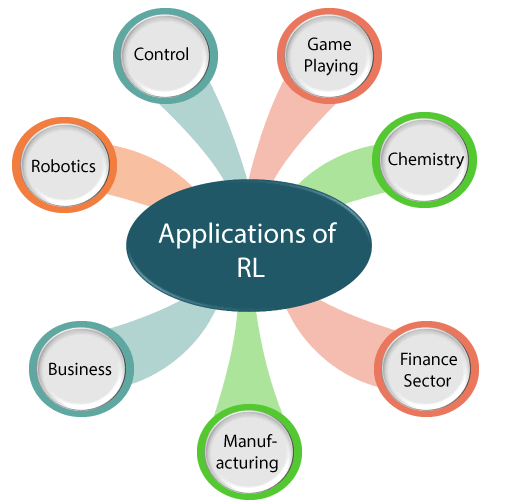
\includegraphics[scale=.5]{5}
	\caption{Minh họa ứng dụng của học tăng cường trong thực tế}
\end{figure}
\section{Bài toán chiếc Taxi thông minh}
\subsection{Bài toán}
Ta có một chiếc taxi được trang bị các cảm biến, trí tuệ nhân tạo, . . . để có thể tự vận
hành trong mọi điều kiện giao thông và thời tiết. Nhiệm vụ của chiếc xe này là đón và trả
khách tại những vị trí nhất định. Ngoài ra, việc vận chuyển hành khách cần phải thỏa mãn
những tiêu chí sau:
\begin{itemize}
	\item Phải trả khách tại đúng vị trí được chỉ định
	\item Tiết kiệm thời gian cho hành khách một cách tối đa
	\item Đảm bảo hành khách được an toàn và phải tuân thủ tất cả các luật giao thông được đưa
	ra
\end{itemize}
\subsection{Mô hình hóa bài toán}
Trước khi có thể sử dụng các kỹ thuật học tăng cường để huấn luyện cho chiếc taxi (\textit{agent}
của chúng ta) thực hiện công việc đưa đón khách một cách tự động, ta cần phải quan tâm
đến một vài khía cạnh về việc mô hình hóa bài toán. Ta cần phải biết phần thưởng (\textit{rewards}),
không gian trạng thái (\textit{state space}) của chiếc taxi, và các hành động (\textit{actions}) mà chiếc taxi
có thể thực hiện tại mỗi trạng thái.
\subsubsection{Phần thưởng}
Vì chiếc taxi sẽ được huấn luyện bằng cách thử và sai khi tương tác với môi trường, ta
cần phải định nghĩa phần thưởng và/hoặc hình phạt cho nó
\begin{itemize}
	\item Chiếc taxi (\textit{agent}) sẽ nhận được một phần thưởng lớn (+20 điểm) khi trả khách thành
	công (trả đúng vị trí được đưa ra)
	\item Chiếc taxi sẽ bị phạt nặng nếu nó trả khách sai vị trí (-10 điểm)
	\item Chiếc taxi sẽ bị phạt "nhẹ" (\textit{slight negative reward}) trong suốt chuyến hành trình đi
	đến vị trí trả khách (-1 điểm/bước). Hình phạt ở đây không được lớn vì ta không muốn
	việc chiếc taxi cố gắng "lao" đến đích một cách nhanh nhất có thể mà vi phạm luật
	giao thông hay gây nguy hiểm cho hành khách.
\end{itemize}
\subsubsection{Không gian trạng thái}
Không gian trạng thái là tập chứa tất cả những tình huống mà chiếc taxi của chúng ta có
thể gặp phải. Đây là nơi chứa những thông tin vô cùng cần thiết cho chiếc taxi để giúp nó có
thể đưa ra những hành động "đúng" tương ứng với trạng thái mà nó đang ở.\\\\
Giả sử, ta có một bãi tập cho chiếc taxi của chúng ta, như được minh họa trong Hình 3.2;
ở đây, ta sẽ dạy chiếc taxi vận chuyển hành khách đến các vị trí ($R$, $G$, $Y$, $B$) trên bãi tập
\begin{figure}
	\centering
	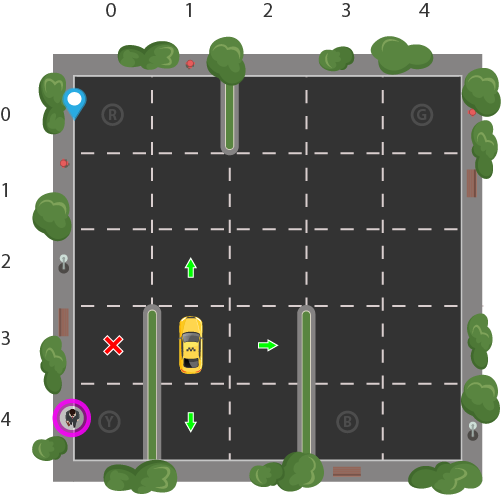
\includegraphics[scale=.5]{7}
	\caption{Mô phỏng taxi trên bãi tập và các vị trí vận chuyển khách}
\end{figure}\\
Để đơn giản hóa bài toán, ta có một số giả định như sau:
\begin{itemize}
	\item Chiếc taxi là phương tiện duy nhất có trên bãi tập
	\item  Khu vực huấn luyện có thể được chia thành một lưới 5 $\times$ 5, cho ta tổng cộng 25 vị trí
	mà chiếc taxi có thể đỗ. Ví dụ, như ta có thể thấy trên Hình 3.2, chiếc taxi đang nằm tại
	vị trí có tọa độ (3, 1); ngoài ra 4 vị trí $R, G, Y, B$ có tọa độ lần lượt là (0,0), (0,4), (4,0),
	(4,3); hành khách đang đứng tại vị trí $Y$ và có mong muốn di chuyển đến
	vị trí $R$ trên bãi tập.
\end{itemize}
Vậy, ta có tổng cộng 5 $\times$ 5 = 25 vị trí mà chiếc taxi có thể xuất hiện, 4 đích đến, và 5 vị
trí của hành khách (4 vị trí tại $R, G, Y, B$ và 1 vị trí là ở trên chiếc taxi). Tổng số trạng thái
có thể có của môi trường sẽ là 5 $\times$ 5 $\times$ 5 $\times$ 4 = 500 trạng thái.
\subsubsection{Không gian hành động}
Tại mỗi thời điểm, chiếc taxi (\textit{agent} của bài toán) sẽ nằm ở 1 trong tổng 500 trạng thái,
và nó sẽ thực hiện một hành động tương ứng với trạng thái hiện có. Hành động ở đây có thể
là đón/trả khách, và di chuyển quanh bãi tập. Không gian hành động của ta sẽ gồm:
\begin{itemize}
	\item Đi lên
	\item Đi xuống
	\item Đi sang trái
	\item Đi sang phải
	\item Đón khách
	\item Trả khách
\end{itemize}
Để ý rằng, tại một số trạng thái ta không thể thực hiện một vài hành động nhất định. Ví
dụ như khi chiếc taxi ở vị trí mép tường bên trái, nó không thể thực hiện hành động đi sang
trái; ta có thể giải quyết vấn đề này bằng việc phạt chiếc taxi khi rơi vào tình huống đó (tình
huống bị "đâm" và tường) và giữ nguyên vị trí hiện tại của nó.
\subsection{Giải quyết bài toán}
Giải pháp được sử dụng để giải quyết bài toán này là giải thuật Q-Learning. Môi trường
của bài toán sẽ được mô phỏng nhờ vào sự trợ giúp của thư viện \textit{Gym} được cung cấp bởi
\textit{OpenAI}.
\\\\Chiếc taxi sẽ được huấn luyện trong 100000 \textit{episode} thông qua việc tương tác với môi
trường. Một vài kết quả trong quá trình huấn luyện được minh họa như trong Hình 3.3, 3.4
và 3.5.
\begin{figure}[h]
	\centering
	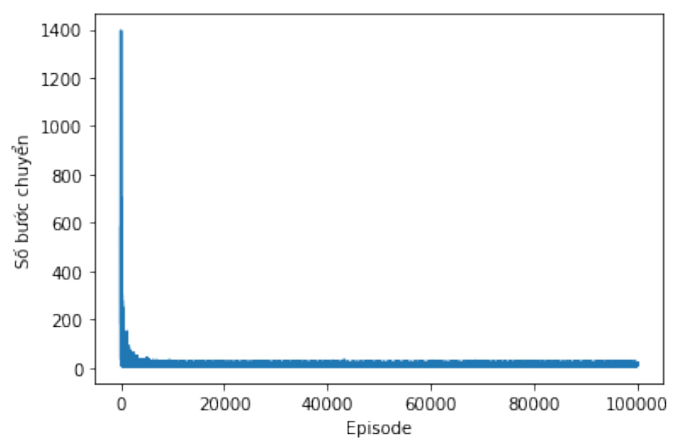
\includegraphics[scale=.6]{9}
	\caption{Số bước chuyển chiếc taxi thực hiện tại mỗi episode.}
\end{figure}
\begin{figure}[h]
	\centering
	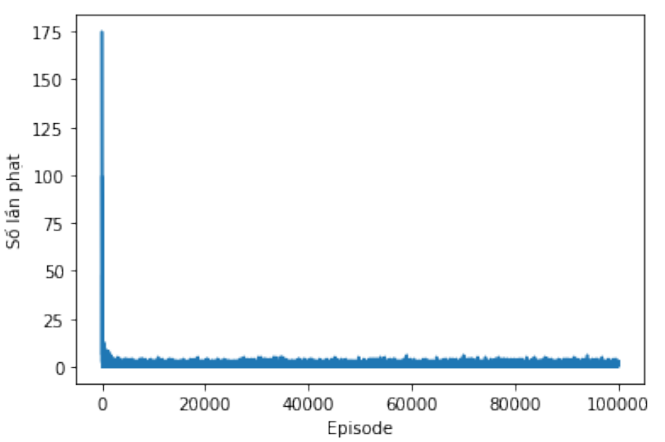
\includegraphics[scale=.6]{10}
	\caption{Số lần chiếc taxi đón/trả khách sai vị trí tại mỗi episode.}
\end{figure}
\begin{figure}[h]
	\centering
	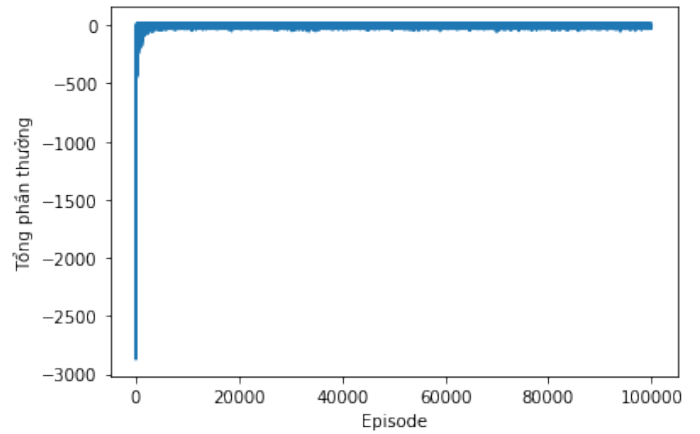
\includegraphics[scale=.6]{11}
	\caption{Số phần thưởng chiếc taxi nhận được tại mỗi episode.}
\end{figure}
\subsection{Kết quả}
Kết quả chạy của bài toán với 1000 \textit{episodes} sau quá trình huấn luyện được minh họa như
trong Hình 3.6
\begin{figure}[h]
	\centering
	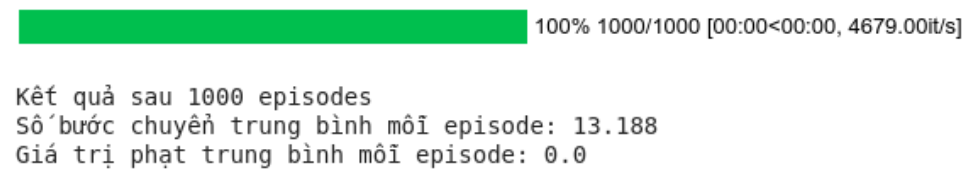
\includegraphics[scale=.5]{12}
	\caption{Kết quả chạy với 1000 episodes.}
\end{figure}
\\Có thể thấy chiếc taxi đã được huấn luyện khá tốt, không mắc bất cứ sai lầm nào trong
việc đón/trả khách và thực hiện việc chọn đường đi khá "thông minh".
\section{Bài toán cân bằng con lắc ngược}
\subsection{Bài toán}
Ta có một con lắc ngược được gắn phía trên một chiếc xe đẩy bằng một khớp nối có thể
quay. Chiếc xe được đặt trên một đường ray không có ma sát và chỉ có thể di chuyển sang
trái hoặc sang phải. Ở trạng thái khởi đầu, con lắc được đặt thẳng đứng, hay nói cách khác
con lắc và đường thẳng vuông góc với đường ray tạo thành một góc $0^\text{o}$. Mục tiêu của bài toán
là không để cho con lắc bị đổ bằng cách tăng hoặc giảm vận tốc của xe đẩy. Trò chơi sẽ kết
thúc khi:
\begin{itemize}
	\item Con lắc bị "đổ" (góc của con lắc nhỏ hơn -12$^\text{o}$ hoặc lớn hơn 12$^\text{o}$),
	\item Hoặc vị trí của xe đẩy năm ngoài đoạn [-2.4, 2.4] (tâm của chiếc xe đẩy đi ra ngoài
	khung nhìn),
	\item Hoặc số bước vượt quá 200.
\end{itemize}
\begin{figure}
	\centering
	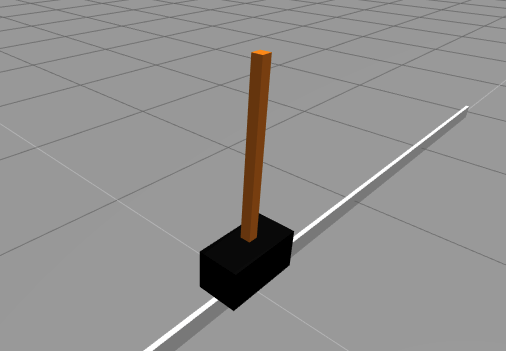
\includegraphics[scale=.6]{8}
	\caption{Minh họa bài toán cân bằng con lắc ngược}
\end{figure}
\subsection{Mô hình hóa bài toán}
\subsubsection{Phần thưởng}
Hệ chuyển động sẽ nhận được phần thưởng +1 sau mỗi bước (bao gồm cả bước kết thúc).
\subsubsection{Không gian trạng thái}
Mỗi trạng thái của hệ sẽ được cấu tạo bởi 4 thành phần:
\begin{itemize}
	\item Vị trí xe đẩy
	\item Vận tốc xe đẩy
	\item Góc của con lắc ngược
	\item Vận tốc ở đỉnh con lắc
\end{itemize}
Miền giá trị của các thành phần này được minh họa như trong bảng dưới đây
\begin{center}
	\begin{tabular}{|c|l|c|c|}
		\hline
		\textbf{Chỉ số} & \textbf{Trạng thái} & \textbf{Min} & \textbf{Max} \\
		\hline
		0 & Vị trí xe đẩy & -2.4 & 2.4 \\
		\hline
		1 & Vận tốc xe đẩy & -Inf & Inf \\
		\hline
		2 & Góc của con lắc ngược & $\sim$-41.8$^\text{o}$ & $\sim$41.8$^\text{o}$ \\
		\hline
		3 & Vận tốc ở định con lắc & -Inf & Inf \\
		\hline
	\end{tabular}
\end{center}
\subsubsection{Không gian hành động}
Có tổng cộng 2 hành động để di chuyển con lắc, đó là đẩy xe sang trái và sang phải.
\subsection{Giải quyết bài toán}
Với số trạng thái quá lớn, việc sử dụng giải thuật Q-Learning như trong bài toán "Chiếc
taxi thông minh" trước đó trở nên bất khả thi về không gian lưu trữ. Việc sử dụng một mạng
nơ-ron nhân tạo (\textit{Artificial Neural Network}) thay thế cho bảng Q-Table có vẻ phù hợp hơn
rất nhiều. 
\begin{figure}[h]
	\centering
	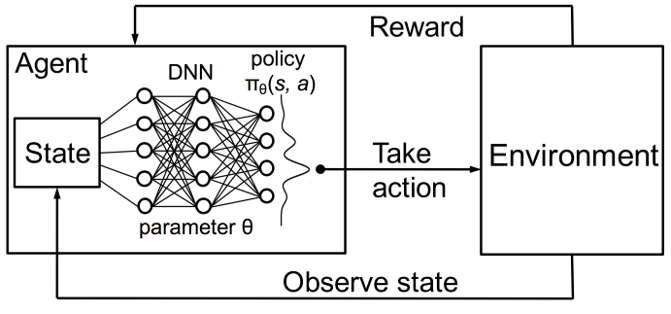
\includegraphics[scale=.6]{15}
	\caption{Mô phỏng lược đồ sử dụng mạng Noron nhân tạo}
\end{figure}

\noindent Hệ xe đẩy con lắc sẽ được huấn luyện trong 60000 \textit{episodes} thông qua việc tương tác với
môi trường. Một vài kết quả trong quá trình huấn luyện được minh họa như trong hình 3.9, 3.10 và 3.11
\begin{figure}[h]
	\centering
	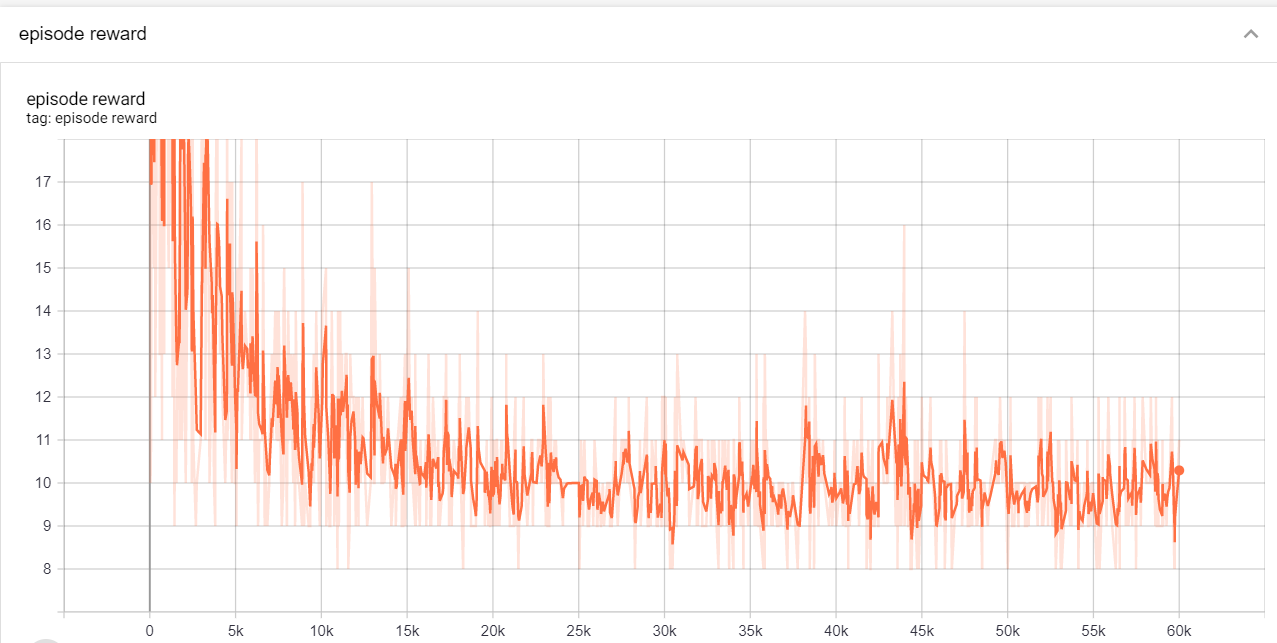
\includegraphics[scale=.3]{16}
	\caption{Tập phần thưởng khi  huấn luyện trong 60000 episodes.}
\end{figure}
\begin{figure}[h]
	\centering
	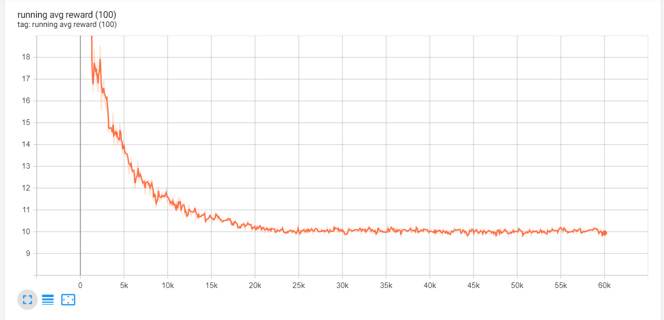
\includegraphics[scale=.75]{17}
	\caption{Số phần thưởng trung bình hệ nhận được qua các episode.}
\end{figure}
\begin{figure}[h]
	\centering
	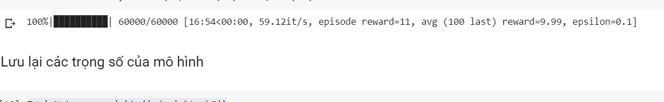
\includegraphics[scale=.75]{18}
	\caption{Kết quả khởi chạy.}
\end{figure}

\chapter{Kết luận và bàn luận}
Trong báo cáo này, nhóm thực hiện đã trình bày sơ lược về quá trình Markov, khái niệm và định nghĩa cơ bản của học tăng cường, các phương pháp liên quan đến quá trình quyết
định Markov, bài toán quyết định Markov và giải thuật Q-Learning.\\\\ Nhóm thực hiện đã đưa ra một số ứng dụng trong thực tế của học tăng cường và lựa chọn hai bài toán cơ bản là Chiếc
taxi thông minh và Bài toán cân bằng con lắc ngược để minh họa cho việc áp dụng những
kiến thức đã được trình bày trong báo cáo.\\\\
Các hướng nghiên cứu tiếp theo của đề tài sẽ tập trung vào các biến thể của thuật toán
Q-Learning cho những bài toán cụ thể khác trong thực tế.

\begin{thebibliography}{}
	\bibitem{latex} J.H Andreae, \textit{Encyclopedia of Infomation Linguistics and Control}, pp.261-270, 1969.
	\bibitem{latex} R.Bellman, \textit{A markovian decision process}, Indiana Univ. Math. J., vol6, pp.679-684, 4 1957, ISSN: 0022-2518.
	\bibitem{latex} D.P. Bertsekas, \textit{Dynamic Programming and Optimal Control}, Athena Scientific; 3 edition (1600), 2005.
		\bibitem{latex}
	https://vi.wikipedia.org/wiki/Học\_tăng\_cường
		\bibitem{latex}
	https://viblo.asia/p/gioi-thieu-ve-hoc-tang-cuong-va-ung-dung-deep-q-learning-choi-game-cartpole-Az45bYy6lxY
	\bibitem{latex}
	https://towardsdatascience.com/reinforcement-learning-lets-teach-a-taxi-cab-how-to-drive-4fd1a0d00529
	\bibitem{latex}
	https://www.theconstructsim.com/testing-different-openai-rl-algorithms-with-ros-and-gazebo/
\end{thebibliography}
\end{document}